%note: don't split this document up with include{...}

\section{Controller}

\subsection{Klassendiagramm}

\begin{figure}[htbp] 
  \centering
  		 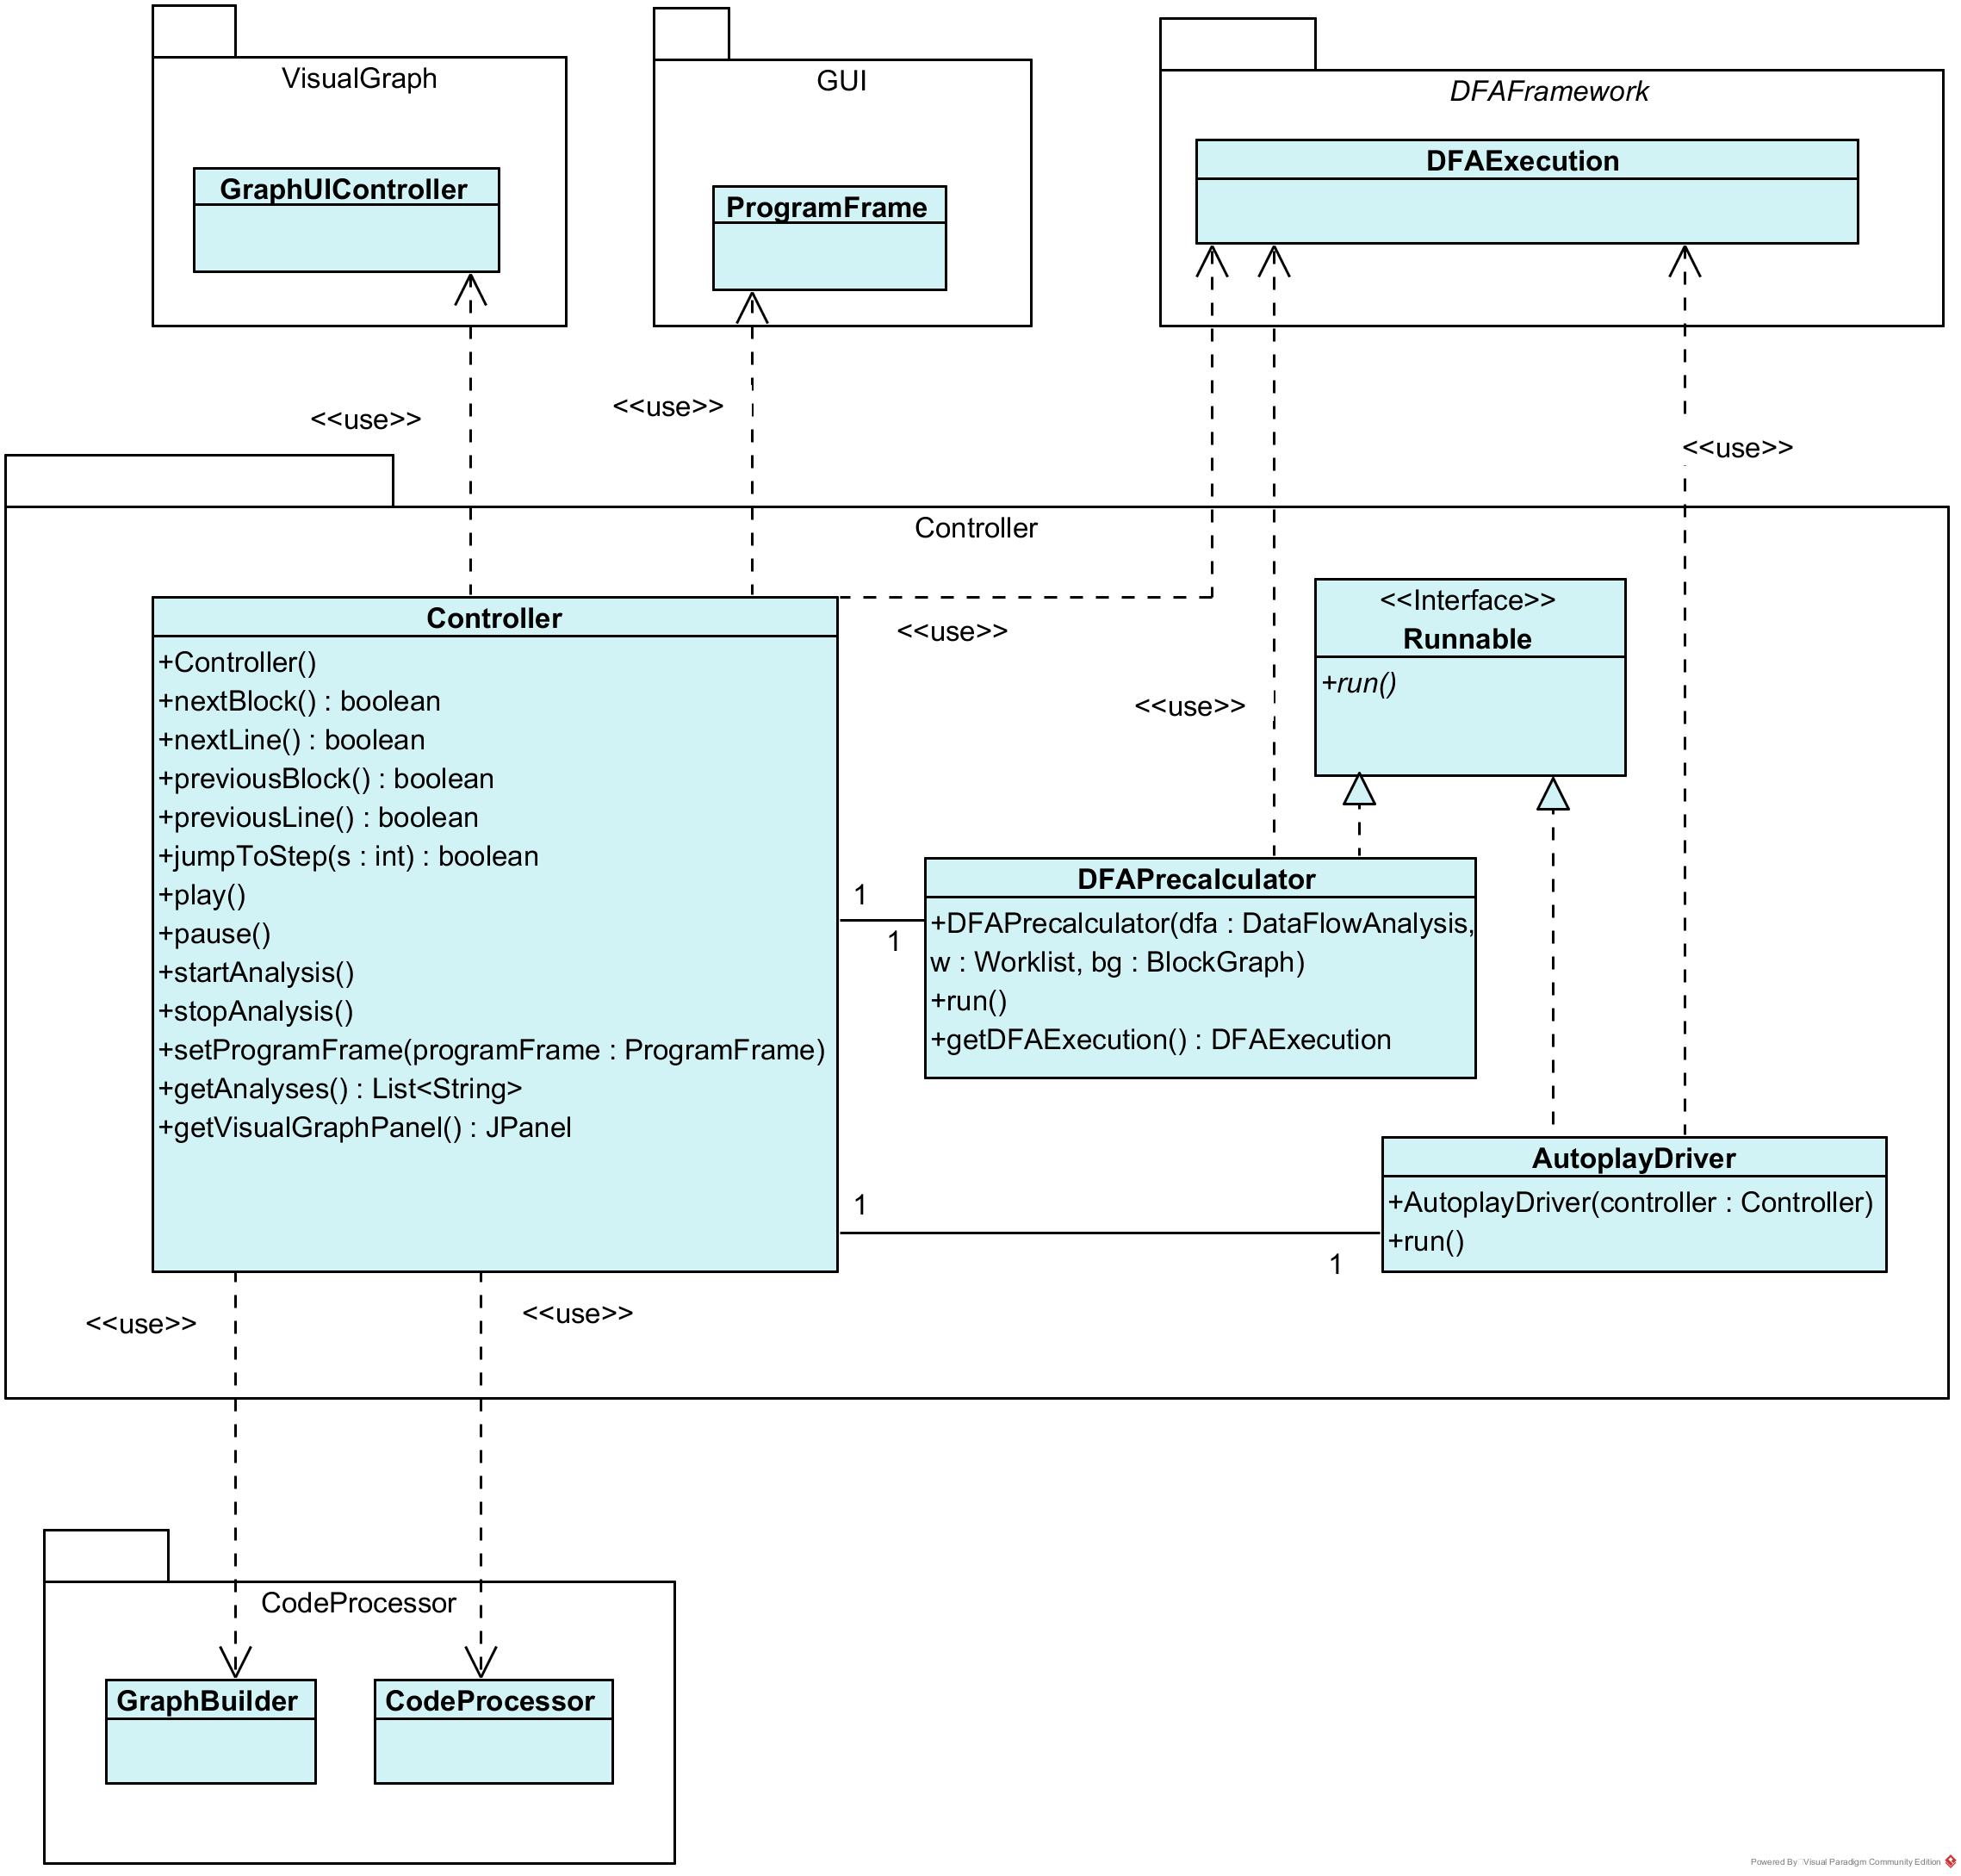
\includegraphics[width=1\textwidth]{Klassenuebersicht/Controller/Controller}
  \caption{Klassendiagramm des User Interfaces}
  \label{fig:UI}
\end{figure}

\subsection{Modulbeschreibung}

Das Controller-Modul ist dafür verantwortlich, die Kommunikation zwischen der Graphischen Benutzeroberfläche (\inlinecode{GUI}) und dem Datenflussanalyse-Framework (DFAFramework) sowie dem CodeProcessor-Modul zu übernehmen.
Außerdem bietet es eine Schnittstelle zum VisualGraph-Modul.

Die Grundidee des \inlinecode{Controllers} basiert auf dem Model-View-Controller Muster (MVC).

Der \inlinecode{Controller} wird benutzt sobald der Benutzer ein GUI-Element benutzt, welches eine Veränderung des Models (\inlinecode{DFAFramework}) nach sich ziehen muss. Darunter fällt zum Beispiel das Starten der Analyse oder die Steuerung der Analyseschritte.
Nicht darunter fällt eine reine Änderung der GUI-Anzeige, wie beispielsweise das Ändern der Größe des Fensters.

Wird nun beispielsweise eine neue Analyse gestartet, so wird der \inlinecode{Controller} von der GUI aufgerufen und beschafft sich alle nötigen Informationen von der GUI.
Dann lässt er den \inlinecode{CodeProcessor} den zu analysierenden Code in einen Kontrollflussgraphen umbauen und gibt diesen dann dem DFAFramework. Dieses berechnet dann die Datenflussanalyse.
Sobald dies abgeschlossen ist, lässt der \inlinecode{Controller} die GUI aktualisieren, wobei er auf dem \inlinecode{GraphUIController} die \inlinecode{start()}-Methode aufruft.
Diese sorgt dafür, dass der Benutzer den Graph im \inlinecode{VisualGraphPanel} sehen kann. Alle anderen Panels steuert der \inlinecode{Controller} selbst an.

Während der Analyse wird der \inlinecode{Controller} weiterhin von der GUI aufgerufen, um die Analyse zu steuern. Der Controller lässt dabei immer das DFAFramework aktualisieren und dann die \inlinecode{GUI} die neuen Informationen anzeigen.

Bei Aktionen die möglicherweise viel Zeit benötigen, erzeugt der \inlinecode{Controller} einen neuen \inlinecode{Thread} um diese Aktion abzuarbeiten.
Dadurch soll die Reaktionsfähigkeit des Programms garantiert werden.

Für den Entwurf ergeben sich folgende Vorteile:
\begin{itemize}
	\item Durch den \inlinecode{Controller} ist die Anwendungslogik klar von den Darstellungen und Benutzerinteraktionen getrennt.
	Dadurch kann die Benutzeroberfläche leicht ausgetauscht werden.
	\item Der Status der Datenflussanalyse kann leicht in unterschiedlichen Darstellungsmodulen repräsentiert werden, wie zum Beispiel als Graph (\inlinecode{VisualGraphPanel}) und als Status eines Knotens (\inlinecode{StatePanel}).
	\item Das bestehende System kann leicht erweitert werden indem neue Teile zum Model (DFAFramework) oder View (GUI) hinzugefügt werden.
\end{itemize}

% the template for one class description
\subsection{Klassenbeschreibung}

\class{Controller}

%Brief descrition of SomeClass.
Die Klasse \inlinecode{Controller} ist für den Großteil der Kommunikation zwischen der GUI und den restlichen Modulen des Programmes zuständig.

\paragraph{Konstruktoren} % skip this if there are no constructors
\begin{itemize}
	\item \ctor{Controller}{}{public}{
		Erzeugt einen \inlinecode{AnalysisLoader} und lädt Analysearten.
		Außerdem wird der \inlinecode{GraphUIController} erzeugt.
	}
\end{itemize}

\paragraph{Methoden}  % skip this if there are no methods
\begin{itemize}
	\item \method{nextBlock}{boolean}{}{public}{
		Wird aufgerufen, sobald in der GUI das entsprechende Event ausgelöst wurde.
		Lässt das DFAFramework den nächsten Block (Knoten des Kontrollflussgraphen) berechnen und sorgt dann dafür, dass der \inlinecode{GraphUIController} das \inlinecode{VisualGraphPanel} aktualisiert.
		
		Gibt \inlinecode{true} zurück, falls dies erfolgreich war, \inlinecode{false} wenn nicht.
	}
	\item \method{nextLine}{boolean}{}{public}{
		Wird aufgerufen, sobald in der GUI das entsprechende Event ausgelöst wurde.
		Lässt das DFAFramework die nächste Zeile innerhalb eines Blocks berechnen, oder springt zum nächsten Block. Danach sorgt er dafür, dass der \inlinecode{GraphUIController} das \inlinecode{VisualGraphPanel} aktualisiert.
		
		Gibt \inlinecode{true} zurück, falls dies erfolgreich war, \inlinecode{false} wenn nicht.
	}
	\item \method{previousBlock}{boolean}{}{public}{
		Wird aufgerufen, sobald in der GUI das entsprechende Event ausgelöst wurde.
		Lässt das DFAFramework den vorherigen Block (Knoten des Kontrollflussgraphen) berechnen und sorgt dann dafür, dass der \inlinecode{GraphUIController} das \inlinecode{VisualGraphPanel} aktualisiert.
		
		Gibt \inlinecode{true} zurück, falls dies erfolgreich war, \inlinecode{false} wenn nicht.
	}
	\item \method{previousLine}{boolean}{}{public}{
		Wird aufgerufen, sobald in der GUI das entsprechende Event ausgelöst wurde.
		Lässt das DFAFramework die vorherige Zeile innerhalb eines Blocks berechnen, oder springt zum Anfang dieses Blocks. Danach sorgt er dafür, dass der \inlinecode{GraphUIController} das \inlinecode{VisualGraphPanel} aktualisiert.
		
		Gibt \inlinecode{true} zurück, falls dies erfolgreich war, \inlinecode{false} wenn nicht.
	}
	\item \method{jumpToStep}{boolean}{s : int}{public}{
		Wird aufgerufen, sobald in der GUI das entsprechende Event ausgelöst wurde.
		Lässt das DFAFramework eine bestimmte Zeile oder einen bestimmten Block berechnen und sorgt dann dafür, dass der \inlinecode{GraphUIController} das \inlinecode{VisualGraphPanel} aktualisiert.
		
		Gibt \inlinecode{true} zurück, falls dies erfolgreich war, \inlinecode{false} wenn nicht.
	}
	\item \method{play}{void}{}{public}{
		Wird aufgerufen, sobald in der GUI das entsprechende Event ausgelöst wurde.
		
		Erzeugt einen \inlinecode{AutoplayDriver}, welcher ein \inlinecode{Thread} ist, der die Schritte der Datenflussanalyse automatisch durchgeht.
		Dies passiert durch mehrmaliges aufrufen der \inlinecode{nextLine()}-Methode (bei eingestelltem Delay größer als 0 Sekunden).
		
		Ruft \inlinecode{jumpToStep()} mit dem letzten Schritt der Analyse auf, falls der Delay auf 0 Sekunden eingestellt ist.
	}
	\item \method{pause}{void}{}{public}{
		Wird aufgerufen, sobald in der GUI das entsprechende Event ausgelöst wurde. 
		Unterbricht den \inlinecode{AutoplayDriver}, sodass der Benutzer wieder manuell alle Schritte durchgehen kann.
		
	}
	\item \method{startAnalysis}{void}{}{public}{
		Wird aufgerufen, sobald in der GUI das entsprechende Event ausgelöst wurde.
		Beschafft sich alle nötigen Informationen von der GUI.
		Lässt dann die \inlinecode{CodeProcessor}-Klasse aus der Benutzereingabe Java-Bytecode kompilieren.
		Dieser wird vom \inlinecode{GraphBuilder} in einen \inlinecode{BlockGraph} umgewandelt und dem  \inlinecode{DFAPrecalculator} zusammen mit einer \inlinecode{Worklist} und einer \inlinecode{DataFlowAnalysis} übergeben, um den Kontrollflussgraphen und die Schritte der Datenflussanalyse vor zu berechnen. Danach wird auf dem \inlinecode{GraphUIController} \inlinecode{start()} aufgerufen, um den Kontrollflussgraphen anzeigen zu lassen.
		
		In der GUI werden das \inlinecode{StatePanel}, das \inlinecode{ControlPanel} und das \inlinecode{VisualGraphPanel} aktiviert. Das \inlinecode{InputPanel} wird deaktiviert.
	}
	\item \method{stopAnalysis}{void}{}{public}{
		Wird aufgerufen sobald in der GUI das entsprechende Event ausgelöst wurde.
		Verwirft die aktuelle \inlinecode{DFAExecution} und lässt den \inlinecode{GraphUIController} den Inhalt des \inlinecode{VisualGraphPanels} löschen.
		Abschließend werden  das \inlinecode{ControlPanel}, das \inlinecode{StatePanel} und das \inlinecode{VisualGraphPanel} deaktiviert und das \inlinecode{InputPanel} aktiviert. 
		
	}
	\item \method{setProgramFrame}{void}{programFrame : ProgramFrame}{public}{
		Übergibt dem \inlinecode{Controller} das \inlinecode{ProgramFrame}.
		Dieser kann darüber auf die GUI-Elemente zugreifen.
	}
	\item \method{getAnalyses}{List<String>}{}{public}{
		Gibt eine Liste mit den Namen der Analysen zurück, welche beim Programmstart vom \inlinecode{AnalysisLoader} gefunden wurden.
	}
	\item \method{getVisualGraphPanel}{JPanel}{}{public}{
		Gibt das \inlinecode{VisualGraphPanel}, welches der \inlinecode{GraphUIController} erstellt hat zurück.
	}
\end{itemize}

\subsubsection{DFAPrecalculator implements Runnable}
%Brief descrition of SomeClass.
Diese Klasse lässt die \inlinecode{DFAExecution} die Datenflussanalyse in einem separaten \inlinecode{Thread} vorberechnen, sodass der Benutzer die Berechnung abbrechen kann falls sie in eine Endlosschleife läuft oder zu viel Speicher verbraucht.


\subparagraph{Konstruktoren} % skip this if there are no constructors
\begin{itemize}
	\item \ctor{DFAPrecalculator}{dfa : DataFlowAnalysis, w : Worklist, bg : Blockgraph}{public}{
		Übergibt dem \inlinecode{DFAPrecalculator} alle nötigen Daten um eine \inlinecode{DFAExecution} zu erzeugen.
	}
\end{itemize}

\subparagraph{Methoden}  % skip this if there are no methods
\begin{itemize}
	\item \method{run}{void}{}{public}{
		Wird beim Starten des \inlinecode{Threads} aufgerufen und lässt die \inlinecode{DFAExecution} vorberechnen.
	}
	
	\item \method{getDFAExecution}{dfae : DFAExecution}{}{public}	{
	Gibt die berechnete \inlinecode{DFAExecution} zurück.
	}
\end{itemize}

\class{AutoplayDriver implements Runnable}
%Brief descrition of SomeClass.
Diese Klasse lässt die einzelnen Schritte der Analyse ablaufen, wenn der Benutzer die Autoplay-Funktion benutzt. Sie arbeitet in einem separaten \inlinecode{Thread}.


\subparagraph{Konstruktoren} % skip this if there are no constructors
\begin{itemize}
	\item \ctor{AutoplayDriver}{controller : Controller}{public}{
		Übergibt dem \inlinecode{AutoplayDriver} eine Instanz der \inlinecode{Controller} Klasse, über welche sie die Schritte der Datenflussanalyse ausführen kann.
	}
\end{itemize}

\subparagraph{Methoden}  % skip this if there are no methods
\begin{itemize}
	\item \method{run}{void}{}{public}{
		Wird beim Starten des \inlinecode{Threads} aufgerufen und lässt die einzelnen Schritte der Analyse abarbeiten.
	}
\end{itemize}